% ---------------------------------------------------------------------------
% Diagrama de bloques del MPSoC Zynq UltraScale+ y de la tarjeta ZCU102 sobre
% la que se ha desarrollado y validado este trabajo: los dominios PS y PL del
% chip, los puertos AXI que los comunican y lo que añade la placa alrededor.
% Fuente del PDF que incluye la memoria (capítulo 2).
%
% Sobre la planta: los rótulos de cada banda van fuera de su recuadro de trazos
% en lugar de encajados en una esquina, que es donde se montaban encima de la
% línea. La banda va más estrecha que antes (16,4 cm en vez de 19,6) para que el
% factor de escala hasta el ancho de caja suba y la letra se lea, y a cambio
% ocupa algo más de alto, que es el reparto que interesa aquí.
%
% Compilar:  pdflatex diagrama_mpsoc_zynq.tex
% ---------------------------------------------------------------------------
\documentclass[border=8pt,12pt]{standalone}
\usepackage[utf8]{inputenc}
\usepackage[T1]{fontenc}
\usepackage{lmodern}
\usepackage{tikz}
\usetikzlibrary{arrows.meta, calc}

\definecolor{cPropio}{HTML}{2A78D6}   % azul: lógica de diseño propio
\definecolor{cIP}{HTML}{EDA100}       % ámbar: IP de terceros
\definecolor{cExt}{HTML}{1BAF7A}      % aguamarina: software y hardware externo
\definecolor{cRef}{HTML}{8A8A85}      % gris: líneas, bandas y contornos

\begin{document}
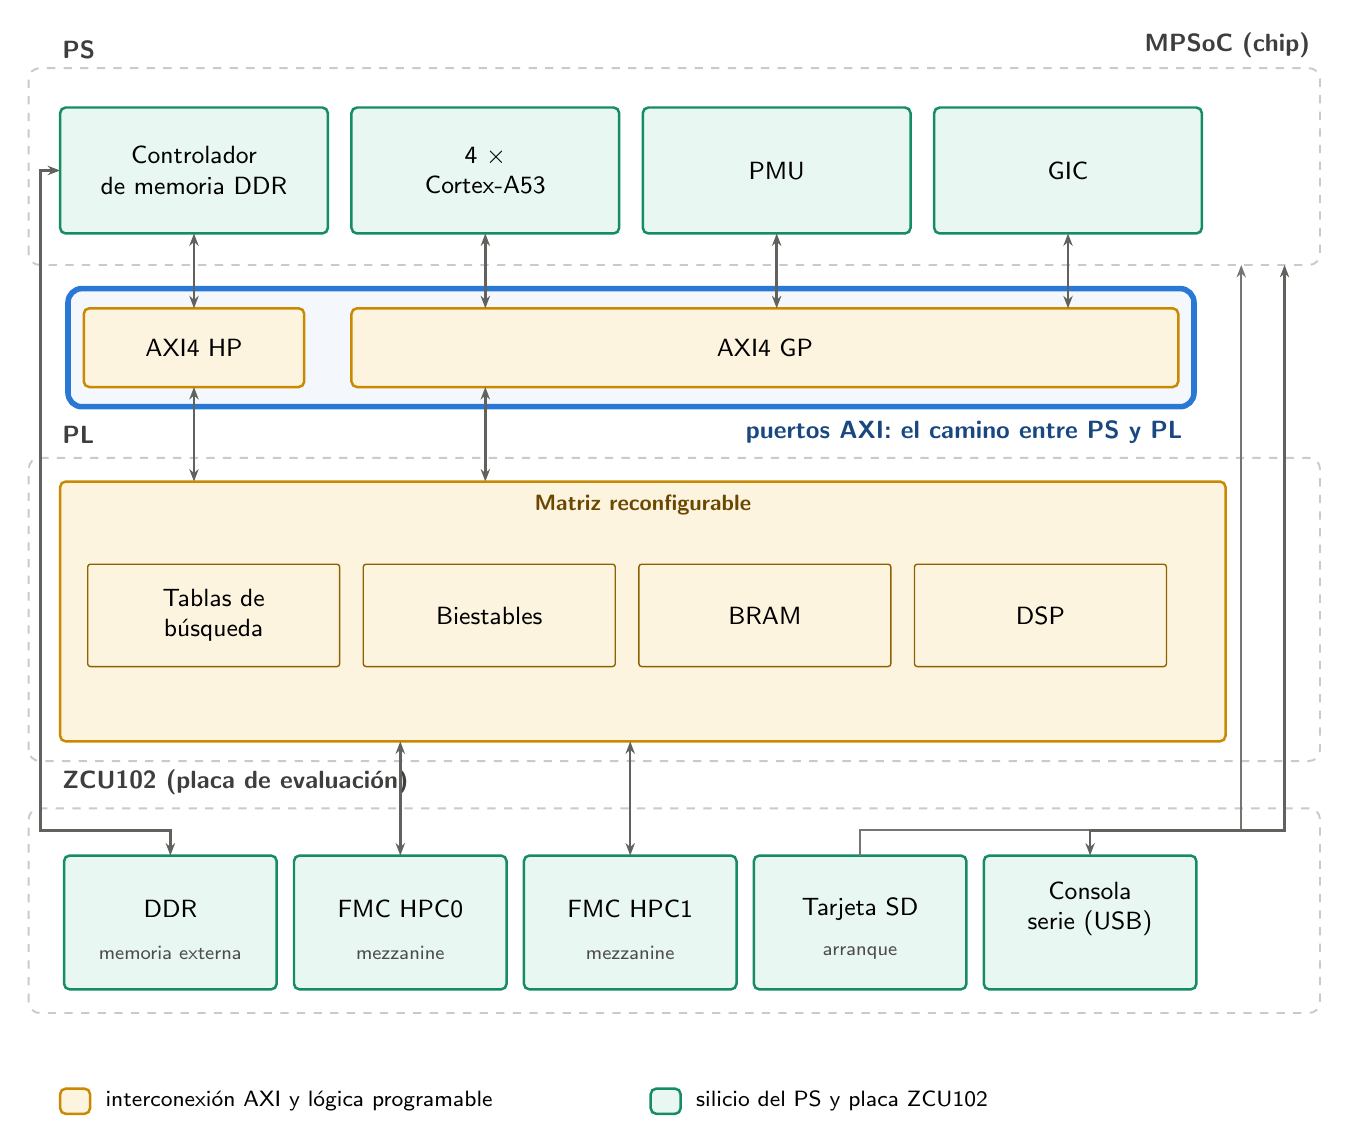
\begin{tikzpicture}[
    x=1cm, y=1cm, font=\sffamily\small,
    blk/.style={draw=cPropio, line width=0.9pt, rounded corners=2pt,
                fill=cPropio!7},
    ip/.style={draw=cIP!85!black, line width=0.9pt, rounded corners=2pt,
               fill=cIP!12},
    ext/.style={draw=cExt!80!black, line width=0.9pt, rounded corners=2pt,
                fill=cExt!10},
    band/.style={draw=cRef!45, dashed, line width=0.7pt, rounded corners=4pt},
    sig/.style={-{Stealth[length=4.5pt]}, line width=0.7pt, cRef!85!black},
    bus/.style={{Stealth[length=4.5pt]}-{Stealth[length=4.5pt]},
                line width=0.9pt, cRef!70!black},
    lbl/.style={font=\sffamily\small, inner sep=2pt},
    sub/.style={font=\sffamily\scriptsize, text=cRef!55!black, inner sep=2pt},
    bandlbl/.style={font=\sffamily\small, text=cRef!45!black, inner sep=2pt},
    leg/.style={font=\sffamily\footnotesize, inner sep=2pt},
]

% ===================== Bandas =====================
\draw[band] (-0.30,9.20) rectangle (16.10,11.70);
\node[bandlbl, anchor=south west] at (0.05,11.75) {\textbf{PS}};
\node[bandlbl, anchor=south east] at (16.05,11.75) {\textbf{MPSoC (chip)}};

\draw[band] (-0.30,2.90) rectangle (16.10,6.75);
\node[bandlbl, anchor=south west] at (0.05,6.85) {\textbf{PL}};

\draw[band] (-0.30,-0.30) rectangle (16.10,2.30);
\node[bandlbl, anchor=south west] at (0.05,2.40)
      {\textbf{ZCU102 (placa de evaluación)}};

% ===================== PS: bloques =====================
\draw[ext] (0.10,9.60) rectangle (3.50,11.20);
\node[align=center] at (1.80,10.40) {Controlador\\de memoria DDR};

\draw[ext] (3.80,9.60) rectangle (7.20,11.20);
\node[align=center] at (5.50,10.40) {4 $\times$\\Cortex-A53};

\draw[ext] (7.50,9.60) rectangle (10.90,11.20);
\node at (9.20,10.40) {PMU};

\draw[ext] (11.20,9.60) rectangle (14.60,11.20);
\node at (12.90,10.40) {GIC};

% ===================== Puertos AXI (entre PS y PL) =====================
% El texto del capitulo manda mirar aqui, asi que la banda va recuadrada y
% rotulada: es el camino que recorren los datos de los catorce enlaces serie.
\draw[draw=cPropio, line width=2pt, rounded corners=5pt, fill=cPropio!5]
      (0.20,7.40) rectangle (14.50,8.90);

\draw[ip] (0.40,7.65) rectangle (3.20,8.65);
\node[lbl] at (1.80,8.15) {AXI4 HP};

\draw[ip] (3.80,7.65) rectangle (14.30,8.65);
\node[lbl] at (9.05,8.15) {AXI4 GP};

\node[lbl, anchor=east, text=cPropio!60!black, fill=white, inner xsep=4pt]
      at (14.50,7.08) {\textbf{puertos AXI: el camino entre PS y PL}};

% Del PS a los puertos, y de los puertos a la matriz.
\foreach \x in {1.80, 5.50, 9.20, 12.90} {\draw[bus] (\x,9.60) -- (\x,8.65);}
\foreach \x in {1.80, 5.50} {\draw[bus] (\x,7.65) -- (\x,6.45);}

% ===================== PL: matriz reconfigurable =====================
\draw[ip] (0.10,3.15) rectangle (14.90,6.45);
\node[leg, text=cIP!45!black] at (7.50,6.15) {\textbf{Matriz reconfigurable}};

\foreach \x/\t in {0.45/{Tablas de\\búsqueda}, 3.95/{Biestables},
                   7.45/{BRAM}, 10.95/{DSP}} {
    \draw[draw=cIP!60!black, line width=0.5pt, rounded corners=1pt]
          (\x,4.10) rectangle (\x+3.20,5.40);
    \node[align=center] at (\x+1.60,4.75) {\t};
}

% ===================== ZCU102: periféricos de la placa =====================
\foreach \x/\t/\s in {0.15/{DDR}/{memoria externa},
                      3.07/{FMC HPC0}/{mezzanine},
                      5.99/{FMC HPC1}/{mezzanine},
                      8.91/{Tarjeta SD}/{arranque},
                      11.83/{Consola\\serie (USB)}/{}} {
    \draw[ext] (\x,0.00) rectangle (\x+2.70,1.70);
    \node[align=center] at (\x+1.35,1.02) {\t};
    \node[sub, anchor=north] at (\x+1.35,0.62) {\s};
}

% ===================== FMC hacia la PL =====================
\draw[bus] (4.42,1.70) -- (4.42,3.15);
\draw[bus] (7.34,1.70) -- (7.34,3.15);

% ===================== DDR: bypass hasta el controlador del PS =====================
\draw[bus] (1.50,1.70) -- (1.50,2.02) -- (-0.15,2.02) -- (-0.15,10.40) -- (0.10,10.40);

% ===================== SD y consola: bypass hasta la banda PS =====================
% Sin rotulo: los dos bloques de origen ya dicen lo que son.
\draw[sig] (10.26,1.70) -- (10.26,2.02) -- (15.10,2.02) -- (15.10,9.20);
\draw[bus] (13.18,1.70) -- (13.18,2.02) -- (15.65,2.02) -- (15.65,9.20);

% ===================== Leyenda =====================
\draw[ip]  (0.10,-1.58) rectangle (0.48,-1.26);
\node[leg, anchor=west] at (0.60,-1.42) {interconexión AXI y lógica programable};
\draw[ext] (7.60,-1.58) rectangle (7.98,-1.26);
\node[leg, anchor=west] at (8.10,-1.42) {silicio del PS y placa ZCU102};

\end{tikzpicture}
\end{document}
